\documentclass{dcctese}
\usepackage[latin1,utf8]{inputenc}  

\usepackage[brazil]{babel}   
\usepackage[T1]{fontenc}   


%\usepackage[portuguese]{babel}
%\usepackage[utf8]{inputenc}
%\usepackage[T1]{fontenc}


%\usepackage{psfig}
\usepackage{a4wide}
\usepackage{comment}
\usepackage[pdftex]{graphicx,color}
\usepackage{graphicx}
\usepackage{graphics}
\usepackage{cite}
\usepackage{longtable}
\usepackage{float}
\usepackage{fancyvrb}
\usepackage{fancyhdr}
\usepackage{setspace}
\usepackage{amsmath}
\usepackage{lscape}

\graphicspath{{../img/}} %path da pasta que contem as imagens

\renewcommand{\topfraction}{1}
\renewcommand{\bottomfraction}{1}
\renewcommand{\floatpagefraction}{1}
\renewcommand{\textfraction}{0}
%\renewcommand{\baselinestretch}{2}  
\doublespacing %espa�amento duplo
\sloppy

\floatstyle{plain}  %%% tipos: plain, boxed, ruled
\newfloat{codigo}{tbp}{lop}[section]
\floatname{codigo}{C\'{o}digo}

%%% nome para ser usado no sum�rio

\newcommand{\listofcodename}{Lista de C\'{o}digos}

\begin{document}

%\onehalfspacing

% folha de titulo / capa------------------------------------------------------------------------------------------------------------------------------------

\thispagestyle{empty}



\title{ \textbf{DESENVOLVIMENTO DE PADR\~{A}O PARA MONOGRAFIAS DE ENGENHARIA DE COMPUTA\c{C}\~{A}O DA UEA}}

\author{ \bf UNIVERSIDADE DO ESTADO DO AMAZONAS - UEA\\[12pt] \bf ESCOLA SUPERIOR DE TECNOLOGIA \\[12pt] \bf ENGENHARIA DE COMPUTA\c{C}\~AO\\ [96pt] NOME DO ALUNO}

%\author{ \bf UNIVERSIDADE DO ESTADO DO AMAZONAS - UEA \\[12pt] \bf ESCOLA SUPERIOR DE TECNOLOGIA \\[12pt] \bf ENGENHARIA DE COMPUTA\c{C}\~{A}O \\
%	[96pt] \bf LANIER MENEZES DOS SANTOS}

\maketitle

\begin{center}
\large Manaus\\
\large 2010
\end{center}

\newpage

% folha de Rosto----------------------------------------------------------------------------------------------------------------------------------------------
\thispagestyle{empty}
\begin{center}
	\textbf{\\[4em]LANIER MENEZES DOS SANTOS \\[5cm]}
	\textbf{DESENVOLVIMENTO DE PADR\~{A}O PARA MONOGRAFIAS DE ENGENHARIA DE COMPUTA\c{C}\~{A}O DA UEA\\[96pt]}
\end{center}
\hspace*{8cm}
\begin{minipage}{8cm} 
	Trabalho de Conclus\~{a}o de Curso apresentado \`{a} banca avaliadora do Curso de Engenharia de Computa\c{c}\~{a}o, da 
	Escola Superior de Tecnologia, da Universidade do Estado do Amazonas, como
	pr\'e-requisito para obten\c{c}\~{a}o do t\'{\i}tulo de Engenheiro de Computa\c{c}\~{a}o.\\[50pt] 
\end{minipage} 
\begin{center}
	Orientador: Prof. M. Sc. Jucimar Maia da Silva J\'{u}nior\\[4ex]
	\normal Manaus\\
	\normal2010
\end{center}
\newpage

% ficha Catalogr�fica------------------------------------------------------------------------------------------------------------------------------------------

\pagenumbering{roman}
\setcounter{page}{2}
\textit{ \textbf{\\ Universidade do Estado do Amazonas - UEA\\Escola Superior de Tecnologia - EST} }
\textit{\\Reitor:\\ \textbf{Nome do Reitor Vigente}\\Vice-Reitor:\\ \textbf{Nome do Vice-Reitor}}
\\
\textit{
Diretor da Escola Superior de Tecnologia:\\ 
\textbf{Nome completo do atual diretor da unidade}}
\\
\textit{
Coordenador do Curso de Engenharia de Computa\c{c}\~{a}o:\\
\textbf{Nome do atual coordenador}}
\\
\textit{
Coordenador da Disciplina Trabalho de Conclus\~ao de Curso:\\
\textbf{Nome do professor da disciplina}}
\\[12pt]
\textit{
Banca Avaliadora composta por: \hfill Data da Defesa: \rule{.5cm}{.1mm}/\rule{.5cm}{.1mm}/\rule{.9cm}{.1mm}.\\
}
\textit{ 
\textbf{Prof. T\'{i}tulo. Nome completo do professor} (Orientador)\\
\textbf{Prof. T\'{i}tulo. Nome completo do professor} \\
\textbf{Prof. T\'{i}tulo. Nome completo do professor} \\
}

\begin{center}\large \bf CIP - Cataloga\c{c}\~{a}o na Publica\c{c}\~{a}o\end{center}
\begin{center}
	\fbox{
		\parbox{17cm}{
			\begin{minipage}{16cm} 
				<C\'{o}digo CIP> \hspace*{1cm} <\'{U}ltimo Nome>, <Primeiro Nome>\\[12pt]
				\hspace*{2cm} \parbox{14cm}{
				\hspace*{0.5cm}<T\'{i}tulo da Monografia>/ 
				<Primeiro> <\'{U}ltimo Nome>; [orientado por] Prof. <T\'{i}tulo>. <Nome do Professor> - Manaus: UEA, <Ano>.\\
				\hspace*{0.5cm}240 p.: il.; 30cm\\
				\hspace*{0.5cm}Inclui Bibliografia\\
				\hspace*{0.5cm}Trabalho de Conclus\~{a}o de Curso (Gradua\c{c}\~{a}o em Engenharia de Computa\c{c}\~{a}o).
				Universidade do Estado do Amazonas, <Ano>.\\[12pt]
				\hspace*{8cm} CDU: \hrulefill}
			\end{minipage}
		}
	}
\end{center}
\newpage

% folha de aprova��o----------------------------------------------------------------------------------------------------------------------------------
\begin{center}
\bf LANIER MENEZES DOS SANTOS\\[1.5 cm]
\end{center}

\begin{center}
\bf DESENVOLVIMENTO DE PADR\~{A}O PARA MONOGRAFIAS DE ENGENHARIA DE COMPUTA\c{C}\~{A}O DA UEA\\[1.5cm]
\end{center}

\hspace*{8cm}
\begin{minipage}{8cm} 

Trabalho de Conclus\~{a}o de Curso apresentado \`{a} 
banca avaliadora do Curso de Engenharia de Computa\c{c}\~{a}o, 
da Escola Superior de Tecnologia, da Universidade do Estado do Amazonas, 
como pr\'e-requisito para obten\c{c}\~{a}o do t\'{\i}tulo de Bacharel em
Engenharia de Computa\c{c}\~{a}o.\\

\large \bf Aprovado em: 00/00/2015
\end{minipage} 

BANCA EXAMINADORA\\[12 pt]

\noindent \hrulefill \hspace*{6cm} \\
\noindent \textbf{Prof. Jucimar Maia da Silva J\'{u}nior, Mestre}\\
\textit{UNIVERSIDADE DO ESTADO DO AMAZONAS}\\[0.5cm]

\noindent \hrulefill \hspace*{6cm} \\
\noindent \textbf{Prof. Nome do Professor, T\'{\i}tulo do Prof.}\\
\textit{UNIVERSIDADE DO ESTADO DO AMAZONAS}\\[0.5cm]

\noindent \hrulefill \hspace*{6cm} \\
\noindent \textbf{Prof. Nome do Professor, T\'{\i}tulo do Prof.}\\
\textit{UNIVERSIDADE DO ESTADO DO AMAZONAS}\\
\let\cleardoublepage\clearpage
%\newpage
% agradecimentos------------------------------------------------------------------------------------------------------------------------------------------------------
% use o prefacio para agradecimentos, dedicat�rias, ...
% o arquivo prefacio deve come�ar com \chapter*{Pref\'{a}cio}
\hspace*{8cm}
\begin{minipage}{8cm}

\vfill
\vskip 20em
\chapter*{Agradecimentos}  %{Pref\'{a}cio}
Ao finalizar este trabalho, ap\'{o}s dois anos e seis meses, tive o
prazer de contar com a amizade e o incentivo de pessoas que
tornaram mais suave este caminho. A elas, agrade\c{c}o:

  Aos meus pais e meu irm\~{a}o, que ficaram privados de minha
  companhia diversas vezes, mas sempre me incentivaram e
  apoioaram.

  \`{A} minha ``fam\'{i}lia'', com quem pude dividir alegrias
  e ang\'{u}stias durante o tempo em que ficamos em na faculade.
\end {minipage}
\newpage

% resumo----------------------------------------------------------------------------------------------------------------------------------------------------------------------

\begin{center} \LARGE \bf Resumo \end{center} 
\vskip 4em

Phasellus fringilla nulla eget nunc adipiscing in volutpat enim bibendum. 
Aliquam et ante at ipsum molestie sodales. Pellentesque mattis venenatis metus, 
at tristique diam ullamcorper a. Nulla non risus et libero accumsan facilisis 
id ac justo. Ut eleifend placerat velit quis vehicula. 

Neste contexto, a metodologia proposta, que envolve a verifica\c{c}\~{a}o formal
do mecanismo de reconhecimento de ondas eletrocardiogr\'aficas e
sequ\^{e}ncias de ondas com a utiliza\c{c}\~{a}o da ferramenta de verifica\c{c}\~{a}o
de modelos {\em Verus}, tem apresentado resultados concretos na
corre\c{c}\~{a}o e projeto deste mecanismo de reconhecimento atrav\'es da
identifica\c{c}\~{a}o e corre\c{c}\~{a}o de falhas, tornando o sistema mais seguro e
confi\'avel.

Aenean metus lectus, iaculis id tincidunt quis, 
tincidunt ut dolor. Integer porttitor tincidunt augue sed condimentum. Mauris pellentesque 
vestibulum justo, vel pellentesque tellus suscipit in. Nulla eget sem augue. 
Vestibulum in sapien nec nibh accumsan ultricies. Aliquam varius consectetur lorem sed luctus. 
Nullam id ipsum ut ante tristique tempor.

A aplica\c{c}\~ao da metodologia permitiu que outras ondas fossem
reconhecidas pelo mecanismo de leitura de dados
eletrocardiogr\'aficos, de forma que fosse feito o
re-projeto do autômato para reconhecimento de ondas, bem como
fosse projetado um aut\^omato para o reconhecimento de sequ\^encias
de ondas, contribuindo de maneira concreta para o desenvolvimento
da aplica\c{c}\~{a}o biom\'edica.


Palavras Chave: Lorem, Ipsum

\newpage

% abstract---------------------------------------------------------------------------------------------------------------------------------------------------------------------

\begin{center} \LARGE \bf Abstract \end{center}
\vskip 4em
\\[2cm]
Curabitur aliquam purus vitae velit elementum sollicitudin eget at turpis. 
Mauris nec mauris ac tortor elementum ultrices. Ut nec nisl arcu. 
Nullam non nunc ante. Donec ac mauris ut nulla vulputate lobortis. 
In ac quam tellus. Vivamus viverra tortor quis lectus dictum malesuada. 

Sed posuere, nunc sed aliquam pharetra, felis massa venenatis justo, 
sed mattis massa magna quis quam. Donec et velit ac orci aliquet blandit. 
Integer sit amet dolor ac sem pretium tincidunt. Nam volutpat convallis elementum. 
Ut accumsan arcu et ipsum accumsan tincidunt.

Cras nec quam mi, ut mattis ante. Lorem ipsum dolor sit amet, consectetur adipiscing elit. 
Sed fringilla auctor dictum. Nam hendrerit sapien sed massa consequat rutrum. 
Nullam congue, augue sed commodo malesuada, lectus nulla mollis magna, eget semper risus 
nisl eget elit. Duis vitae hendrerit massa. In a odio nunc, sit amet mollis dolor. 

In accumsan suscipit dui, a vestibulum diam condimentum ullamcorper. Etiam ut quam arcu, 
ac tristique ante. Vestibulum imperdiet elit non ante tristique accumsan. Donec vulputate 
fringilla tempor. Proin porttitor nisi nisi. Fusce vel ullamcorper orci. Lorem ipsum dolor 
sit amet, consectetur adipiscing elit. 

Key-words: Lorem, Ipsum


\newpage

% sum�rio-----------------------------------------------------------------------------------------------------------------------------------------------------------------------
\renewcommand{\contentsname}{Sum\'{a}rio}
\tableofcontents
\listoftables
\newpage

\listoffigures
\addcontentsline{toc}{chapter}{\listofcodename}
\listof{codigo}{\listofcodename}  % Lista de C�digos

\clearpage

% inicio da defini��o dos cabe�alhos--------------------------------------------------------------------------------------------------------------------------------------------
\pagestyle{fancy}
\renewcommand{\chaptermark}[1]{\markboth{#1}{}}
\renewcommand{\sectionmark}[1]{\markright{#1}}
\renewcommand{\headrulewidth}{0.5pt}
\newcommand{\rom}{\fontfamily{cmr}\fontseries{m}\fontsize{10}{12}\selectfont}
\fancyhf{} \fancyhead[LE,RO]{\rom\thepage}
\fancyhead[LO]{\rom\rightmark} \fancyhead[RE]{\rom\leftmark}
\fancypagestyle{plain}{
    \fancyhead{} % get rid of headers
    \renewcommand{\headrulewidth}{0pt} % and the line
 }
% fim dos cabe�alhos------------------------------------------------------------------------------------------------------------------------------------------------------------

% inicio do texto---------------------------------------------------------------------------------------------------------------------------------------------------------------

\pagenumbering{arabic}

% os arquivos de cada capitulo devem iniciar com \chapter{Nome do Capitulo}
% (o nome deve terminar com .tex)

%% Introdu��o
\chapter {Como Escrever Uma monografia}\label{cap:comoEscrever}

\section{Ao Candidato}

O texto abaixo foi livremente adaptado de \cite{COMER2010} para ajudar os alunos a escreverem suas monografias. 

Se você está se preparando para escrever uma monografia em uma área experimental da Engenharia da Computação. 
A menos que você tenha escrito muitos documentos formais antes, você tem uma surpresa: isso é difícil!

Existem dois caminhos possíveis para o sucesso:

\begin{itemize}
	\item Planejamento
	
	Poucas pessoas pegam esse caminho. As poucas que pegam, deixam a universidade tão rápido, 
	que eles malmente são notados. Se você quer fazer a impressão final e ter uma longa carreira como um 
	estudante de graduação, não escolha este caminho.
	
	\item Perseverança
	
	Tudo que você tem que fazer é sobreviver à sua banca julgadora. 
	A boa notícia é que eles são bem mais velhos que você, assim você pode adivinhar quem vai eventualmente 
	``expirar''  primeiro (morrer).
	A má notícia é que é que eles são mais experientes nesse jogo (afinal, eles perseveraram na frente da banca deles, não!?).
	
\end{itemize}
	
Aqui estão algumas linhas-guia que podem ajudá-lo quando você finalmente levar a sério escrever. 
A lista segue infinitamente; você provavelmente não vai querer ler isso tudo de uma vez. Mas, por favor, leia isso antes de 
escrever qualquer coisa.

\hfill

\section{A Idéia Geral}	

\begin{enumerate}
	
	\item Uma monografia é um documento formal onde o aluno descreve a realização de um trabalho técnico onde usou as técnicas e conceitos aprendidos durante o curso de 	graduação.

	\item Em geral, toda afirmação em uma monografia deve ser embasada ou por uma referência em literatura científica publicada ou por um trabalho original.
	Acima de tudo, uma monografia não repete os detalhes do pensamento crítico e análises encontradas nas fontes publicadas; usa o resultado como fato e 
	referencia o leitor às fontes para mais detalhes. 

	\item Cada sentença em uma monografia deve ser completa e correta gramaticalmente. Além do mais, a monografia deve satisfazer estritamente as 
	regras da gramática formal (e.x., sem contrações, sem coloquialismo, sem pronúncias erradas, sem jargão técnico indefinido, sem piadas escondidas e sem gírias,
	mesmo quando tais termos ou frases são de comum uso na língua falada). Realmente, a escrita de uma monografia deve ser um cristal limpo.
	Sombras de significados importam; a terminologia e a prosa devem fazer uma fina distinção. As palavras devem carregar exatamente o sentido pretendido, nada mais e nada 	menos.

	\item Cada afirmação em uma monografia deve ser correta e defensível no sentido lógico e científico. Acima de tudo, as discussões em uma monografia devem satisfazer
	a maioria das estritas regras de lógica aplicada à matemática e Engenharia.                       

\end{enumerate}

\section{O que se Deve Aprender do Exercício}

\begin{enumerate}

	\item Todo engenheiro precisa comunicar descobertas; a monografia fornece um treinamento para comunicação com outros engenheiros.

	\item Escrever uma monografia requer que o estudante pense profundamente, para organizar a discussão técnica, para reunir argumentos que convencerão outros engenheiro,
	e seguir as regras para uma rigorosa apresentação dos argumentos e discussões.

\end{enumerate}

\section{Regra do Polegar}

Boa escrita é essencial para uma monografia. Entretanto, boa escrita não pode compensar uma escassez de idéias ou conceitos.
Pelo contrário, uma apresentação limpa sempre expõe fraquezas.

\section{Definições e Terminologia}

\begin{enumerate}

	\item Cada termo técnico usado em uma monografia deve ser definido ou por uma referência à uma definição publicada anteriormente (para termos padrões com seus significados usuais)
	ou por uma precisa, não-ambígua definição que aparece antes do termo ser usado (para termos novos ou um termo padrão usado de maneira não usual).

	\item Cada termo deve ser usado de uma e única maneira por toda monografia.			

	\item A forma mais fácil de evitar uma longa série de definições é incluir uma afirmação: ``a terminologia usada no decorrer deste documento segue a mesma dada em [CITAÇÃO].''
	Então, só defina exceções.

	\item O capítulo introdutório pode dar o intuito (i.e., definições informais) dos termos fornecidos, os quais serão mais precisamente definidos depois.

\end{enumerate}

\section{Termos e Frase a Evitar}
	
\begin{itemize}

	\item Advérbios

		\indent Na maioria das vezes, são ``muito frequentemente usados demais''. Ao invés deles use palavras mais fortes. Alguém pode dizer, por exemplo, `` Escritores abusam de advérbios.''
	
	\item Piadas ou Trocadilhos

		\indent Esses não têm lugar em um documento formal.
	
	\item ``Ruim'', ``Bom'', ``Terrível'', ``Estúpido''

		\indent Uma monografia não faz julgamento moral. Use ``incorreto/correto'' para se referir à erros ou corretudes de fato.
		Use palavras precisas ou frases para avaliar qualidade (e.x. ``método A requer menos recurso computacional que método B''). Em geral, deve-se evitar todos os julgamentos qualitativos.
		
	\item ``Verdade'', ``Puro''

		\indent No mesmo senso de ``bom'' (é um julgamento).
		
	\item ``Perfeito''

		\indent Nada é.
		
	\item ``Uma solução ideal''

		\indent Você está julgando de novo.
		
	\item ``Hoje'', ``Tempos modernos''

		\indent Hoje é o ontem de amanhã.
		
	\item ``Logo''

		\indent Logo quanto? Hoje à noite? Próxima década?
		
	\item ``Estávamos surpresos ao ver ...''

		\indent Mesmo se você estivesse, e daí?
		
	\item ``Parece'', ``Aparentemente''

		\indent Não importa como algo aparenta.
	
	\item ``Parece mostrar''

		\indent Tudo o que importa são os fatos.
		
	\item ``Em termos de''

		\indent Normalmente vago.
		
	\item ``Baseado em'', ``X-baseado'', ``Como base de''

		\indent Cuidado, pode ser vago.
		
	\item ``Diferente''

		\indent	Não significa ``vários''. Diferente do que?
		
	\item ``Na luz de''

		\indent	Coloquial. 
		
	\item ``Um monte de''

		\indent	Vago & Coloquial
		
	\item ``Tipo de''

		\indent	Vago & Coloquial
		
	\item ``Algo como''

		\indent	Vago & Coloquial
		
	\item ``Mais ou Menos'' 

		\indent	Vago & Coloquial
		
	\item ``Número de''

		\indent	Vago, você quer dizer, ``alguns'', ``muitos'' ou ``a maioria''? Uma afirmação quantitativa é preferível.
		
	\item ``Devido a''

		\indent	Coloquial
		
	\item ``Provavelmente''

		\indent	Apenas se você souber a probabilidade estatística (se você sabe, afirme quantitativamente).
		
	\item ``Obviamente'', ``Claramente''

		\indent Tenha cuidado: Óbvio/Claro para todos?
		
	\item ``Simples''

		\indent Pode ter uma conotação negativa, como em ``simplório''.
		
	\item ``Junto com''

		\indent Use somente ``com''.
		
	\item ``Na verdade'', ``Realmente''

		\indent Defina os termos claramente para eliminar a necessidade de esclarecimento.
		
	\item ``O fato de''

		\indent Faz uma meta-sentença; reformule a frase.
		
	\item ``Isso'', ``Aquilo''

		\indent Como em ``Estas causa envolvem.'' Razão: ``Isso'' pode referir ao sujeito da sentença anterior, à toda sentença anterior, todo o parágrafo anterior, toda a seção anterior, etc. 
		Mais importante, pode ser interpretado no sentido correto ou no meta-sentido. Por exemplo: \textit{``X faz Y. Isso significa...''} o leitor pode assumir ``isso'' referindo ao 			
		\textit	{Y} ou ao fato de \textit{X faz Y}. Mesmo quando restrito (e.x., ``esta computação''), a frase é fraca e frequentemente ambígua.
		
	\item ``Você irá ler sobre isso''

		\indent A segunda pessoa não tem lugar em uma monografia.
		
	\item ``Eu vou descrever''

		\indent A primeira pessoa não tem lugar em uma monografia formal. Se auto-referência é essencial, escreva como ``Seção 10 descreve...''
		
	\item ``Nós'' como em ``Vemos que''

		\indent Uma armadilha a evitar. Razão: Quase toda sentença pode ser escrita para começar com ``nós'' porque `nós'' pode se referir: ao leitor e autor, ao autor e consultor, ao autor e grupo de pesquisa, engenheiros de computação, a toda comunidade de Engenharia da computação, ou algum outro grupo não especificado. 

	\item ``Esperançosamente, o programa''

		\indent Programas não tem esperança, não até serem implementados com sistemas de IA. Aliás, se você estiver escrevendo uma tese de IA, fale com outra pessoa: pessoas de IA tem seus próprios sistemas de regras.
		
	\item ``...um famoso pesquisador...''

		\indent Não importa quem disse ou fez. De fato, tais afirmações prejudicam o leitor.
		
	\item Tenha cuidado usando: ``poucos, maioria, todos, algum, cada'' 

		\indent Uma monografia é precisa. Se a sentença diz ``Maioria dos sistemas computacionais contém X'', você deve ser capaz de defender isso. Você tem certeza que conhece os fatos? Quantos computadores foram construídos e vendidos ontem?
		
	\item ``Deve'', ``Sempre''

		\indent Absolutamente?
		
	\item ``Deveria''

		\indent Quem disse isso?
		
	\item ``Prova'', ``Comprova''

		\indent Um matemático aceitaria que isso é uma prova?

	\item ``Pode'', ``Poderia''

		\indent Sua mãe provavelmente lhe disse a diferença.

\end{itemize}

\section{Voz}

Use construções ativas. Por exemplo, diga ``o sistema operacional inicia o dispositivo'' ao invés de ``o dispositivo é iniciado pelo sistema operacional.''

\section{Tempo Verbal}

Escreva no presente. ``O sistema escreve a página no disco e então usa o frame...'' ao invés de ``O sistema usará o frame depois de ter escrito a página no disco...''

\section{Defina Negações com Antecedência}

Exemplo: diga ``Nenhum bloco de dados espera na fila de saída'' ao invés de ``Um bloco de dados esperando saída não está na fila.''

\section{Gramática e Lógica}

Tenha cuidado pois o sujeito de cada sentença realmente faz o que o verbo diz q ele faz. 
Dizer ``Programas devem fazer chamada de processo usando a instrução X'' não é o mesmo que dizer ``Programas devem usar a instrução X quando chamam um procedimento.'' 
De fato, a primeira é evidentemente falsa! 
Outro exemplo: ``RPC requer programas para transmitir pacotes grandes'' não é o mesmo que ``RPC requer um mecanismo que permita programas transmitirem pacotes grandes.''

\section{Foco nos Resultados e não nas Pessoas/Circunstâncias em que Foram Obtidos}
		
``Depois de trabalhar oito horas no laboratório naquela noite. nós percebemos...'' não tem lugar na monografia. 
Não importa quando você percebeu isso, ou quanto tempo você trabalhou para obter a resposta. 
Outro exemplo: ``Jim e eu chegamos aos números mostrados na tabela 3 medindo...'' Ponha um agradecimento para Jim na monografia, mas não inclua nomes (nem mesmo o seu) no corpo principal. 
Você pode estar tentado a documentar uma longa série de experimentos que não produziram nada ou uma coincidência que resultou em sucesso. Evite completamente isso. 
Em particular, não documente aparentemente influências místicas (e.x., ``se aquele gato não tivesse rastejado pelo buraco no chão, poderíamos 
não ter descoberto o indicador de erro do fornecimento de energia na ponte de rede''). Nunca atribua tais eventos à causas místicas ou dê a 
entender que forças estranhas podem ter afetado seu resultado. 
Resumo: Prenda-se nos fatos evidentes. Descreva os resultados sem mencionar suas reações ou eventos que o ajudaram a alcançá-los.

\section{Evite Auto-Avaliação (Elogio e Crítica)}

Ambos os exemplos a seguir estão incorretos: ``O método esboçado na Seção 2 representa o maior avanço em design de sistemas distribuídos porque...'' 
``Embora a técnica na próxima seção não seja extraordinário,...''

\section{Referências à Trabalhos}

Sempre cita-se o artigo, não o autor. Assim, usa-se um verbo no singular para referir ao artigo, mesmo que tenha muitos autores. Por exemplo ``Johnson e Smith [Johnson and Smith1995] relata que...''
Evite a frase `` os autores afirmam que X''. O uso de ``afirmam'' lança dúvida em ``X'' porque referencia os pensamentos do autor ao invés dos fatos. Se você concorda ``X'' está correto, simplesmente escreva ``X'' seguido da referência. Se absolutamente deve referenciar um artigo ao invés do resultado, diga ``o artigo afirma que'' ou ``Johnson e Smith [Johnson and Smith1995] apresentam evidências que...''

\section{Conceito Vs. Exemplo}

Um leitor pode ficar confuso quando um conceito e um exemplo deste estão embaçados. 
Exemplos comuns incluem: um algoritmo e um programa particular que o implementa, uma linguagem de programação e um compilador, uma abstração geral e sua implementação 
particular em um sistema de computador, uma estrutura de dados e uma instância particular em memória.

\section{Terminologia para Conceitos e Abstrações}

Quando definir a terminologia para um conceito, tenha cuidado para decidir precisamente como a idéia se traduz para uma implementação. Considere a seguinte discussão:
\textit{Sistemas VM incluem um conceito conhecido como endereço de espaço. O sistema cria dinamicamente um endereço de espaço quando um programa precisa de um, e destrói um endereço de espaço 
quando o programa que criou o espaço terminar de usá-lo. Um sistema VM usa um pequeno, finito número para identificar cada endereço de espaço. 
Conceitualmente, entende-se que cada endereço de espaço deveria ter um novo identificador. Entretanto, se um sistema VM executa por um tempo que esgote todos os possíveis identificadores de endereços de espaço, 
ele deve reusar um número}
O ponto importante é que a discussão só faz sentido porque define ``endereço de espaço'' independente de ``identificador de endereço de espaço''. 
Se espera-se discutir as diferenças entre um conceito e sua implementação, as definições devem permitir tal distinção.

\section{Conhecimento Vs. Dados}

O fato que resulta de um experimento é chamado ``dado''. 
O termo ``conhecimento'' implica que o fato tenha sido analisado, condensado ou combinado com fatos de outros experimentos para produzir informação útil.

\section{Causa e Efeito}

Uma monografia deve separar cuidadosamente causa-efeito de simples correlações estatísticas. Por exemplo, mesmo se todos os programas de computador escritos no laboratório do Professor X requerem mais memória que os programas escritos no laboratório do Professor Y, isso pode não ter nada a ver com os professores ou laboratórios ou programadores (e.x., talvez as pessoas que trabalham no laboratório do Professor X estejam trabalhando em aplicações que requerem mais memória do que no laboratório do Professor Y).

\section{Descreva Somente Conclusões Comprovadas}   		

Deve-se ter cuidado para apenas escrever conclusões que as evidências suportam. Por exemplo, se programas executam muito mais lento no computador A do que no computador B, 
não pode-se concluir que o processador de A é mais lento que o de B a menos que se tenha anotado todas as diferenças entre os sistemas operacionais dos computadores, dispositivos de entrada e saída, 
tamanho de memória, memória cache, ou largura de banda do barramento interno. 
De fato, deve-se ainda abster-se de julgamentos a menos que se tenha os resultados de um experimento controlado (e.x., executando uma lista de vários programas muitas vezes, cada um quando o computador 
estiver ocioso). Mesmo se a causa de algum fenômeno parece óbvia, não pode-se dar uma conclusão sem sólida evidência embasada.

\section{Comércio e Ciência}

Em uma monografia, nunca se escreve conclusões sobre viabilidade econômica ou sucesso comercial de uma idéia/método, nem faz-se especulações sobre a história do desenvolvimento ou origens de
uma idéia. Um engenheiro deve permanecer objetivo sobre os méritos de uma idéia, independente de sua popularidade comercial. Em particular, um engenheiro nunca assume que o sucesso comercial é uma medida válida 
de mérito (muitos produtos populares não são nem bem projetados nem bem construídos). Assim, afirmações tais como ``mais de quatrocentos vendedores fazem produtos usando a técnica Y'' são irrelevantes em uma monografia.

\section{Política e Ciência}

Um engenheiro evita toda influência política quando está avaliando Idéias. Obviamente, não deveria importar se grupos governamentais, grupos políticos, grupos religiosos ou outras organizações aprovam uma idéia.
Mais importante e frequentemente despercebida, não importa se uma idéia uma idéia foi originada por um engenheiro que já tenha ganho um premio Nobel ou um aluno no primeiro ano de graduação. Deve-se avaliar a idéia independente da fonte.

\section{Organizações Canônicas}
 	
Em geral toda monografia deve definir o problema que motivou a pesquisa, contar por que este problema é importante, contar o que outros fizeram, descrever as novas contribuições, documentar os experimentos que validam a contribuição e fazer conclusões.
Não existe organização canônica para uma monografia; cada uma é única. Entretanto, novatos que escrevem uma monografia em uma área experimental da Engenharia da Computação podem achar os seguintes exemplos um bom ponto de início: 

\begin{itemize}
	
	\item \textbf{Capítulo 1: Introdução}

	Uma visão do problema; por que isso é importante; um resumo de um trabalho já existente e uma afirmação de suas hipóteses ou questões específicas a serem exploradas. Faça com que seja legível pra qualquer um.

	\item \textbf{Capítulo 2: Definições}

	Somente termos novos. Faça as definições precisas, concisas e não-ambíguas.

	\item \textbf{Capítulo 3: Modelo Conceitual}

	Descreva o conceito central que influencia o seu trabalho. Faça disso um ``tema'' que amarram todos os seus argumentos. Isso deveria fornecer uma resposta para a questão apresentada na introdução em um nível conceitual. Se necessário, adicione outro capítulo para dar um raciocínio adicional sobre o problema ou sua solução.

	\item \textbf{Capítulo 4: Medidas Experimentais}

	Descreva o resultado experimental que forneça evidências para embasar sua tese. Normalmente experimentos enfatizam prova-ou-conceito (demonstrando a viabilidade de um método/técnica) ou eficiência (demonstrando que um método/técnica proporciona uma performance melhor do que as que já existem)
	
	\item \textbf{Capítulo 5: Resultados e Consequências}

	Descreva variações, extensões ou outras aplicações da idéia central.

	\item \textbf{Capítulo 6: Conclusões}

	Resumo do que foi aprendido e como isso pode ser aplicado. Mencione as possibilidades para pesquisas futuras.

	\item \textbf{Resumo/Abstract}

	Um pequeno (poucos parágrafos) resumo da monografia. Descreva o problema e a abordagem da pesquisa. Enfatize as contribuições originais.

\end{itemize}

\section{Ordem Sugerida para Escrever}

A maneira mais fácil de construir uma monografia é de dentro para fora. Comece escrevendo os capítulos que descrevem sua pesquisa (3, 4 e 5 nas linhas acima). Colete termos como eles surgem no texto e dê uma definição para cada um.
Defina cada termo técnico,  mesmo que você o use de maneira convencional.

Organize as definições em um capítulo separado. Faça as definições precisas e formais. Reveja depois os capítulos para verificar que cada uso de termo técnico adere à uma definição. Depois de ler os capítulos do meio para verificar terminologia, escreva a conclusão. escreva a Introdução logo depois da Conclusão. Finalmente, complete o resumo/abstract.

\section{A Chave do Sucesso}

Aliás, existe uma chave para o sucesso: prática. ninguém nunca aprendeu a escrever lendo composições como esta. Ao invés disso, você precisa praticar, praticar, praticar. Todo dia.

\section{Pensamentos de Despedida}

Nos despedimos de você com as seguintes Idéias para meditar. Se não significarem nada para você agora, visite-as novamente depois de ter escrito sua monografia.

	

	\indent\indent Depois de grande dor, chega um pensamento formal.

		\indent \indent \indent --Emily Dickinson

		
	\indent\indent Um homem pode escrever a qualquer hora, se ele se mantiver persistente para tal.

		\indent \indent \indent --Samuel Johnson

		
	\indent\indent Permaneça perfeito até o final da estrada.

		\indent \indent \indent --Harry Lauder

	 
	\indent\indent Uma típica tese de Ph.D. é nada mais que transferir ossos de um cemitério para outro.

		\indent \indent \indent --Frank J. Dobie

	
	
	
	
	
	
	
	








	
	
	
	
	
	
	
	
	
	
	
	
	
	


%% T�tulo do Capitulo 2
\chapter{Manual do Trabalho de Conclus\~{a}o de Curso - TCC - I e II}
\label{cap:manual TCC}


\section{Trabalho de Conclus\~{a}o de Curso (TCC)}

O TCC \'{e} o \'{u}ltimo e mais importante trabalho de disciplina a ser desenvolvido pelo aluno, individualmente, 
no Curso de Gradua\c{c}\~{a}o de Engenharia da Computa\c{c}\~{a}o. O aluno, orientado por um professor, ter\'{a} oportunidade de demonstrar e por em pr\'{a}tica 
os conhecimentos adquiridos durante o curso, al\'{e}m de aperfei\c{c}oar e comprovar o aprendizado te\'{o}rico e metodologias que lhe foram ensinadas.

O TCC consiste em duas etapas a serem realizadas em semestres distintos:

	\begin{enumerate}
		\item \textbf{TCC}-I: Elabora\c{c}\~{a}o e defesa da monografia.
		O aluno deve documentar, na forma de monografia, toda a fundamenta\c{c}\~{a}o te\'{o}rica e modelagem (se aplic\'{a}vel), de acordo com o tema proposto.
		
		\item \textbf{TCC}-II: Ap\'{o}s aprova\c{c}\~{a}o do TCC-I o aluno dever\'{a} concluir a monografia ao implementar a modelagem proposta ou outro instrumento que possibilite a avalia\c{c}\~{a}o do trabalho face aos objetivos definidos. A defesa inclui a documenta\c{c}\~{a}o finalizada e demonstra\c{c}\~{a}o do que foi desenvolvido (implementa\c{c}\~{a}o).
	\end{enumerate}
	
O TCC, do curso de Engenharia da Computa\c{c}\~{a}o, corresponde a um total de quatro (04) cr\'{e}ditos, a serem efetivados mediante matr\'{i}cula, sendo que dois (02) cr\'{e}ditos ser\~{a}o cumpridos na disciplina TCC-I e dois (02) cr\'{e}ditos na disciplina  TCC-II. 


\subsection{Do Professor da Disciplina}

O TCC funciona como uma disciplina e, portanto, possui um professor respons\'{a}vel, o qual encaminha para avalia\c{c}\~{a}o os trabalhos finais (TCC-I e TCC-II) e controla as notas finais. 

Compete ao professor da disciplina:

	\begin{itemize}
		\item Estabelecer reuni\~{a}o inicial com os alunos e professores para expor as normas do TCC e dar-lhes ci\^{e}ncia desse documento

		\item Divulgar e fazer cumprir as normas referentes ao TCC
		
		\item Divulgar o calend\'{a}rio referente \`{a}s atividades do TCC

		\item Penalizar o aluno pelo n\~{a}o cumprimento dos prazos determinados no calend\'{a}rio de atividades do TCC; (0,2 pts, na m\'{e}dia final, por dia de atraso na entrega 		da proposta e monografia)
		
		\item Divulgar aos alunos a rela\c{c}\~{a}o de professores e suas respectivas linhas de pesquisa para exercerem a atividade de orienta\c{c}\~{a}o
		
		\item Coordenar a forma\c{c}\~{a}o das duplas orientador/orientando

		\item Coordenar o processo de substitui\c{c}\~{a}o orientador/orientando
		
		\item Coordenar o processo de constitui\c{c}\~{a}o das bancas e definir o cronograma de apresenta\c{c}\~{a}o dos trabalhos
		
		\item Encaminhar aos membros da banca o respectivo trabalho para avalia\c{c}\~{a}o
		
		\item Convidar, quando poss\'{i}vel, um avaliador externo para integrar a banca
		
		\item Providenciar os documentos necess\'{a}rios ao processo de avalia\c{c}\~{a}o

		\item Providenciar as declara\c{c}\~{o}es aos professores participantes da banca, bem como do orientador
		
		\item Encaminhar uma c\'{o}pia definitiva do trabalho (TCC-II) \'{a} Biblioteca
		
	\end{itemize}


\subsection{Professor Orientador}

O professor orientador tem a fun\c{c}\~{a}o de ajudar o aluno no direcionamento do seu trabalho, sem, entretanto, desenvolver partes desse 
trabalho para o aluno. O orientador, apenas sugere caminhos que o aluno dever\'{a} seguir, acompanha seu trabalho, motivando e corrigindo eventuais erros.

Antes de apresentar o TCC-I ou TCC-II, o aluno deve submet\^{e}-lo previamente, \textbf{e obrigatoriamente}, \`{a} aprecia\c{c}\~{a}o de seu orientador. 
Dado o aval do mesmo, a proposta poder\'{a} ser encaminhada e apresentada para avalia\c{c}\~{a}o.

Compete ao Professor Orientador:

	\begin{itemize}
		\item Informar ao professor da disciplina a linha de pesquisa que ir\'{a} atuar
	
		\item Orientar a elabora\c{c}\~{a}o do Trabalho de Conclus\~{a}o
	
		\item Auxiliar o aluno na resolu\c{c}\~{a}o de problemas conceituais, t\'{e}cnicos e de relacionamento decorrentes da atividade
	
		\item Estabelecer o plano e cronograma de trabalho em conjunto com o orientando
	
		\item Informar o orientando sobre as normas, procedimentos e crit\'{e}rios de avalia\c{c}\~{a}o respectivos
	
		\item Informar ao aluno, caso haja atraso no cronograma de trabalho ou o n\~{a}o cumprimento das orienta\c{c}\~{o}es, se o trabalho tem condi\c{c}\~{o}es ou n\~{a}o de ser 
		encaminhado para avalia\c{c}\~{a}o
	
		\item liberar o trabalho para que haja a apresenta\c{c}\~{a}o do aluno bem como informar ao professor da disciplina quanto \`{a} apresenta\c{c}\~{a}o do aluno (Anexo C)
	
		\item Rubricar as 3 (tr\^{e}s) vias encaminhadas para avalia\c{c}\~{a}o (TCC-I ou TCC-II) quando estiver ciente e de acordo, 
		conforme suas orienta\c{c}\~{o}es, do material entregue
	
		\item Presidir a banca examinadora do trabalho por ele orientado
	
		\item Comunicar ao professor da disciplina situa\c{c}\~{o}es que exijam provid\^{e}ncias, assim que ocorrerem.
	\end{itemize}


\subsection{Co-orientador}

	\begin{itemize}	
		\item Ser\'{a} solicitado formalmente pelo orientador a Professor da disciplina e ser\'{a} designado por esse para atender quest\~{a}o espec\'{i}fica do trabalho
		
		\item Trabalhar\'{a} em conjunto ao orientador e desempenhar\'{a} papel solicitado pelo mesmo.
	\end{itemize}


\subsection{Orientando}

Compete ao Orientando:

	\begin{itemize}
		\item Comparecer \`{a}s reuni\~{o}es marcadas pelo professor da disciplina sobre o Trabalho de Conclus\~{a}o
		
		\item Escolher a tem\'{a}tica a ser trabalhada em conson\^{a}ncia com as linhas de pesquisa do curso
		
		\item Contatar professor para definir orientador e informar a Coordena\c{c}\~{a}o do Projeto (entrega do Anexo-B)
		
		\item Cumprir as datas limites determinadas no calend\'{a}rio de atividades do TCC. O n\~{a}o cumprimento dos prazos ser\'{a} penalizado com perda de pontua\c{c}\~{a}o; 
		(0,2 pts, na m\'{e}dia final, por dia de atraso na entrega da monografia)
		
		\item Comparecer \`{a}s orienta\c{c}\~{o}es sobre o trabalho; o n\~{a}o comparecimento de tr\^{e}s (03) orienta\c{c}\~{o}es seguidas implica em reprova\c{c}\~{a}o por falta
		
		\item Seguir as orienta\c{c}\~{o}es do professor designado \`{a} orienta\c{c}\~{a}o
		
		\item Cumprir o plano e o cronograma de trabalho elaborado em conjunto com o professor-orientador
		
		\item Comunicar ao professor da disciplina toda e qualquer situa\c{c}\~{a}o que possa comprometer, de alguma forma, o processo de elabora\c{c}\~{a}o, bem como, a conclus\~{a}o do 			trabalho o quanto antes, para que a coordena\c{c}\~{a}o possa analisar o ocorrido e tomar as provid\^{e}ncias cab\'{i}veis
		
		\item Comparecer perante a banca na data, hora e local estabelecido para a realiza\c{c}\~{a}o da sess\~{a}o de avalia\c{c}\~{a}o do TCC
	\end{itemize}


\subsection{Os Acompanhamentos de Orienta\c{c}\~{a}o}

As reuni\~{o}es de orienta\c{c}\~{a}o dever\~{a}o ser documentadas conforme modelo presente no Anexo A e ser\~{a}o entregues ao professor da disciplina no dia da entrega da carta (ANEXO A) solicitando defesa de TCC.
Tanto professor orientador como orientando dever\~{a}o ter uma c\'{o}pia dos acompanhamentos de orienta\c{c}\~{a}o.
	

\subsection{A Banca Examinadora}

A banca examinadora do TCC-I e TCC-II, dever\'{a} ser composta por, no m\'{i}nimo, 3 professores. A banca ser\'{a} constitu\'{i}da pelo 
professor orientador e por dois outros professores. Se houver co-orienta\c{c}\~{a}o, o professor co-orientador pode compor a banca, contudo sua avalia\c{c}\~{a}o n\~{a}o computar\'{a} nota para o alunosua avalia\c{c}\~{a}o n\~{a}o computar\'{a} nota para o aluno 

Os membros da banca examinadora poder\~{a}o sugerir altera\c{c}\~{o}es no trabalho (parte escrita e/ou implementa\c{c}\~{a}o). Para o TCC-I as altera\c{c}\~{o}es dever\~{a}o ser feitas, com o acompanhamento do orientador, para que sejam inclu\'{i}das no trabalho e avaliadas no TCC-II. Para o TCC-II, estas dever\~{a}o ser feitas at\'{e} duas semanas depois da apresenta\c{c}\~{a}o (ver data limite), supervisionadas pelo professor-orientador, para constar no(s) volume(s) final(is) do TCC, que ficar\'{a} \`{a} disposi\c{c}\~{a}o na biblioteca

O volume final para arquivamento (TCC-II) s\'{o} ser\'{a} aceito pela coordena\c{c}\~{a}o de TCC se estiver validado pelo professor orientador, indicando sua concord\^{a}ncia com o conte\'{u}do do mesmo, e a assinatura do aluno


\subsection{Semin\'{a}rios}
Conforme calend\'{a}rio os semin\'{a}rios destinados aos alunos matriculados em TCC, abordam temas que auxiliar\~{a}o na elabora\c{c}\~{a}o do documento escrito e na defesa.

Ser\~{a}o e semin\'{a}rios:
	\begin{itemize}
		\item Semin\'{a}rio I - Estrutura do Trabalho de Conclus\~{a}o de Curso

		\item Semin\'{a}rio II - Normas ABNT

		\item Semin\'{a}rio III - Apresenta\c{c}\~{a}o do TCC (defesa e material)
	\end{itemize}

A participa\c{c}\~{a}o do aluno nos semin\'{a}rios \'{e} um dos crit\'{e}rios que consta na ata de avalia\c{c}\~{a}o. O n\~{a}o comparecimento acarretar\'{a} perda de 0,2 pt por semin\'{a}rio.


\subsection{As Datas Limite}

As datas limites ser\~{a}o estabelecidas e divulgadas de acordo com o calend\'{a}rio acad\^{e}mico de cada per\'{i}odo acad\^{e}mico.


\subsection{Nota Final}

Para aprova\c{c}\~{a}o do aluno no TCC, o mesmo dever\'{a}:

	\begin{itemize}
		\item Atender \`{a} exig\^{e}ncia da frequ\^{e}ncia m\'{i}nima de 75$\%$ (setenta e cinco) \`{a}s orienta\c{c}\~{o}es. 
		A frequ\^{e}ncia do aluno ser\'{a} validada a partir do formul\'{a}rio de acompanhamento de reuni\~{a}o de orienta\c{c}\~{a}o os quais devem ser preenchidos a cada acompanhamento, 			pelo orientador e pelo aluno

		\item Obter, no m\'{i}nimo, grau 6,0 (seis). Este grau ser\'{a} composto pela m\'{e}dia aritm\'{e}tica das avalia\c{c}\~{o}es dos membros da banca examinadora. Cada membro da banca 			receber\'{a} uma planilha com itens a avaliar (por notas). Ao t\'{e}rmino da defesa ser\'{a} preenchida uma ata final de avalia\c{c}\~{a}o de TCC constando a m\'{e}dia final do aluno.
		Caso o aluno n\~{a}o alcance grau m\'{i}nimo seis (6,0) dever\'{a} matricular-se novamente na disciplina para desenvolver novamente o trabalho ou concluir o 			desenvolvimento do mesmo
	\end{itemize}


\section{Trabalho de Conclus\~{a}o de Curso I (TCC-I)}

O aluno, em parceria com um professor orientador, deve delimitar um tema, a ser abordado, dentro das linhas de pesquisa do curso.

Deve ent\~{a}o dar in\'{i}cio \`{a} documenta\c{c}\~{a}o de seu trabalho elaborando uma monografia com os cap\'{i}tulos contendo a fundamenta\c{c}\~{a}o te\'{o}rica e modelagem da implementa\c{c}\~{a}o do trabalho proposto. Ao final do semestre defend\^{e}-lo \`{a} uma banca examinadora.

\subsection{Estrutura do TCC-I}

Na monografia, o aluno dever\'{a} documentar seu trabalho para ser arquivado e, no futuro, referenciado por outras pessoas, lembrando sempre que Trabalho de Conclus\~{a}o de Curso deve ser escrito tendo em vista uma metodologia cient\'{i}fica. 

A monografia deve seguir a seguinte estrutura: 
	
	\indent \textbf{Capa} \\
	\indent \textbf{Folha de Rosto} \\
	\indent \textbf{Ficha para Cataloga\c{c}\~{a}o} (deve ser impressa no verso da folha de rosto) \\
	\indent \textbf{Ep\'{i}grafe} (opcional) \\
	\indent \textbf{Dedicat\'{o}ria} (opcional) \\
	\indent \textbf{Agradecimentos} (opcional) \\
	\indent \textbf{Resumo} \\
	\indent \textbf{Abstract} (resumo em ingl\^{e}s) \\
	\indent \textbf{Sum\'{a}rio} \\
	\indent \textbf{Lista de Figuras} (opcional) \\
	\indent \textbf{Lista de Tabelas} (opcional) \\
	\indent \textbf{Lista de Abreviaturas e siglas} \\
	\indent \textbf{Introdu\c{c}\~{a}o} \\
	\indent \textbf{Desenvolvimento} \\
	\indent \textbf{Conclus\~{a}o} \\
	\indent \textbf{Refer\^{e}ncias Bibliogr\'{a}ficas} \\
	\indent \textbf{Obras Consultadas} \\
	\indent \textbf{Anexos e/ou Ap\^{e}ndices} (opcional) \\\\

\textbf{Introdu\c{c}\~{a}o} - \'{e} o primeiro cap\'{i}tulo da monografia. Apresenta o contexto do trabalho proposto com a defini\c{c}\~{a}o do problema, os objetivos (geral e espec\'{i}ficos), os motivos que levaram \`{a} decis\~{a}o de se abordar o tema e a organiza\c{c}\~{a}o do trabalho.

\textbf{Desenvolvimento} - corresponde aos demais cap\'{i}tulos da monografia, que descrevem sobre o tema proposto, revis\~{a}o da literatura, metodologia aplicada, ferramentas e modelagem (se aplic\'{a}vel) do trabalho a ser implementado.

\textbf{Conclus\~{a}o} - como o TCC-I \'{e} o in\'{i}cio da monografia n\~{a}o ser\'{a} poss\'{i}vel uma conclus\~{a}o, portanto devem ser apresentadas as dificuldades encontradas, at\'{e} o momento no trabalho, e resultados esperados do trabalho proposto.

A formata\c{c}\~{a}o (margens, espa\c{c}amentos, cita\c{c}\~{o}es, pagina\c{c}\~{a}o, etc.) de todo o documento, deve estar voltada para um trabalho cient\'{i}fico, portanto, 
os alunos devem seguir o modelo de monografia adotado pelo curso e dispon\'{i}vel no site do mesmo. 
Solicitamos ainda aos alunos que utilizem as obras abaixo:

	\begin{itemize}	
		\item  FURAST\'{E}, Pedro Augusto. Normas T\'{e}cnicas para o Trabalho Cient\'{i}fico (Nova ABNT). 14 edi\c{c}\~{a}o. Porto Alegre, 2006.

		\item SILVA, Edna L\'{u}cia da. Metodologia da Pesquisa e Elabora\c{c}\~{a}o de Disserta\c{c}\~{a}o - 3ed. rev. e atual. – Florian\'{o}polis: Laborat\'{o}rio de Ensino a Dist\^{a}ncia da 			UFSC, 2001.

		\item BRASIL, ABNT - Associa\c{c}\~{a}o Brasileira de Normas T\'{e}cnicas. NBR 14724.

		\item BRASIL, ABNT - Associa\c{c}\~{a}o Brasileira de Normas T\'{e}cnicas. NBR 10520.

		\item BRASIL, ABNT - Associa\c{c}\~{a}o Brasileira de Normas T\'{e}cnicas. NBR 6023.
	\end{itemize}
	

\subsection{Avali\c{c}\~{a}o do TCC-I}

O TCC-I dever\'{a} ser apresentado perante uma banca examinadora a ser definida pelo professor da disciplina, para a qual o aluno apresentar\'{a} seu trabalho, desde a justificativa do problema que o levou a desenvolv\^{e}-lo at\'{e} as discuss\~{o}es do material levantado.

O aluno ter\'{a} 25 (vinte e cinco) minutos para defesa de sua proposta, onde utilizar\'{a} os recursos audiovisuais que achar necess\'{a}rio e ser\~{a}o utilizados mais 10 (dez) minutos para responder aos questionamentos de cada membro da banca avaliadora. A banca ser\'{a} constitu\'{i}da pelo professor orientador (presidente) e por dois outros professores, podendo ser um convidado externo. Avaliado o trabalho escrito e ``ouvidas'' as sugest\~{o}es da banca, o aluno dever\'{a} fazer as modifica\c{c}\~{o}es necess\'{a}rias.

No TCC-I caso o aluno n\~{a}o alcance grau m\'{i}nimo 6,0 (seis) dever\'{a} matricular-se novamente na disciplina pra desenvolver novamente o trabalho (ou concluir o desenvolvimento do mesmo)  em TCC-I.
\'{e} necess\'{a}rio que o aluno seja aprovado em TCC-I para a conclus\~{a}o do trabalho em TCC-II. 


\section{Trabalho de Conclus\~{a}o de Curso II (TCC-II)}

O aluno dever\'{a} por em pr\'{a}tica a modelagem apresentada em TCC-I al\'{e}m de concluir a monografia (implementa\c{c}\~{a}o, resultados obtidos, etc.). Haver\'{a} nova defesa da documenta\c{c}\~{a}o e demonstra\c{c}\~{a}o do que foi desenvolvido (implementa\c{c}\~{a}o) de acordo com esta documenta\c{c}\~{a}o.


\subsection{Estrutura do TCC-II}

Apresenta a mesma estrutura do TCC-I. Entretanto, no TCC-II, o aluno ir\'{a} complementar a monografia de acordo com as solicita\c{c}\~{o}es feitas pela banca examinadora (na defesa do TCC-I) e com t\'{o}picos relacionados \`{a} sua implementa\c{c}\~{a}o. 

A monografia deve seguir a seguinte estrutura: 

	\indent \textbf{Capa} \\
	\indent \textbf{Folha de Rosto} \\
	\indent \textbf{Ficha para Cataloga\c{c}\~{a}o} (deve ser impressa no verso da folha de rosto) \\
	\indent \textbf{Ep\'{i}grafe} (opcional) \\
	\indent \textbf{Dedicat\'{o}ria} (opcional) \\
	\indent \textbf{Agradecimentos} (opcional) \\
	\indent \textbf{Resumo} \\
	\indent \textbf{Abstract} (resumo em ingl\^{e}s) \\
	\indent \textbf{Sum\'{a}rio} \\
	\indent \textbf{Lista de Figuras} (opcional) \\
	\indent \textbf{Lista de Tabelas} (opcional) \\
	\indent \textbf{Lista de Abreviaturas e siglas} \\
	\indent \textbf{Introdu\c{c}\~{a}o} \\
	\indent \textbf{Desenvolvimento} \\
	\indent \textbf{Conclus\~{a}o} \\
	\indent \textbf{Refer\^{e}ncias Bibliogr\'{a}ficas} \\
	\indent \textbf{Obras Consultadas} \\
	\indent \textbf{Anexos e/ou Ap\^{e}ndices} (opcional) \\\\


\textbf{Introdu\c{c}\~{a}o} - \'{e} o primeiro cap\'{i}tulo da monografia. Apresenta o contexto do trabalho proposto com a defini\c{c}\~{a}o do problema, os objetivos (geral e espec\'{i}ficos), os motivos que levaram \`{a} decis\~{a}o de se abordar o tema e a organiza\c{c}\~{a}o do trabalho.

\textbf{Desenvolvimento} - corresponde aos demais cap\'{i}tulos da monografia, que descrevem sobre o tema proposto, revis\~{a}o da literatura, metodologia aplicada, ferramentas e modelagem (se aplic\'{a}vel) do trabalho a ser implementado.

\textbf{Conclus\~{a}o} - se os objetivos foram atingidos, dificuldades encontradas e sugest\~{o}es para trabalhos futuros.

A formata\c{c}\~{a}o (margens, espa\c{c}amentos, cita\c{c}\~{o}es, pagina\c{c}\~{a}o, etc.) de todo o documento, deve estar voltada para um trabalho cient\'{i}fico, portanto, 
os alunos devem seguir o modelo de monografia adotado pelo curso e dispon\'{i}vel no site do mesmo. 
Solicitamos ainda aos alunos que utilizem as obras abaixo:

	\begin{itemize}	
		\item  FURAST\'{e}, Pedro Augusto. Normas T\'{e}cnicas para o Trabalho Cient\'{i}fico (Nova ABNT). 14 edi\c{c}\~{a}o. Porto Alegre, 2006.

		\item SILVA, Edna L\'{u}cia da. Metodologia da Pesquisa e Elabora\c{c}\~{a}o de Disserta\c{c}\~{a}o - 3ed. rev. e atual. - Florian\'{o}polis: Laborat\'{o}rio de Ensino a Dist\^{a}ncia da 			UFSC, 2001.

		\item BRASIL, ABNT - Associa\c{c}\~{a}o Brasileira de Normas T\'{e}cnicas. NBR 14724.

		\item BRASIL, ABNT - Associa\c{c}\~{a}o Brasileira de Normas T\'{e}cnicas. NBR 10520.

		\item BRASIL, ABNT - Associa\c{c}\~{a}o Brasileira de Normas T\'{e}cnicas. NBR 6023.
	\end{itemize}


\subsection{Avalia\c{c}\~{a}o do TCC-II}

O TCC-II dever\'{a} ser apresentado perante uma banca examinadora a ser definida pelo professor da disciplina, para a qual o aluno apresentar\'{a} seu trabalho, desde a justificativa do problema que o levou a desenvolv\^{e}-lo at\'{e} as discuss\~{o}es do material levantado e a conclus\~{a}o.

Esta apresenta\c{c}\~{a}o dever\'{a} ser, necessariamente, oral e descritiva, onde o aluno dever\'{a} tamb\'{e}m na parte oral resumir as principais fun\c{c}\~{o}es do sistema, o modo como ser\'{a} usado na organiza\c{c}\~{a}o ou ambiente e os seus benef\'{i}cios.

Para esta apresenta\c{c}\~{a}o oral, o aluno dever\'{a} preparar o que ir\'{a} falar e utilizar recursos did\'{a}ticos, considerando o tempo de 45 minutos; cada membro da banca avaliadora ter\'{a} 10 minutos para questionamentos.

N\~{a}o ser\~{a}o aceitas justificativas para a n\~{a}o demonstra\c{c}\~{a}o das implementa\c{c}\~{o}es, implicando assim em reprova\c{c}\~{a}o.

As apresenta\c{c}\~{o}es dos TCCs s\~{a}o abertas ao p\'{u}blico interessado. Sugere-se, fortemente, que os alunos de TCC-I assistam \`{a}s bancas de seus colegas de TCC-II, como experi\^{e}ncia.

Caso o aluno n\~{a}o alcance a nota m\'{i}nima de 6,0 pontos em TCC-II, dever\'{a} matricular-se, novamente na disciplina, no pr\'{o}ximo semestre.
	
A nota do aluno s\'{o} ser\'{a} lan\c{c}ada mediante entrega de 2 c\'{o}pias da vers\~{a}o revisada com visto do orientador, j\'{a} incluindo as modifica\c{c}\~{o}es sugeridas pela banca, no formato final (impresso em jato de tinta ou laser), em capa dura, na cor preta, bem como um CD com a vers\~{a}o final do trabalho e os produtos resultantes da pesquisa, quando for o caso.

	


%% T�tulo do Capitulo 3
\chapter{Título do Terceiro Capítulo}
\label{cap:titulo do terceiro capitulo}

Lorem ipsum dolor sit amet, consectetur adipiscing elit. Quisque turpis risus, pulvinar quis pellentesque vel, sodales a lorem. Nulla eget ante a odio pretium consequat id at odio. Maecenas mauris dolor, laoreet eu consequat sed, mollis sed sapien. Integer dolor nisl, malesuada consectetur vestibulum id, faucibus ac elit. Donec leo justo, consectetur ut suscipit vel, rutrum ac mauris. Sed ut augue tellus. Vestibulum ante ipsum primis in faucibus orci luctus et ultrices posuere cubilia Curae; Integer ac diam sed urna tristique lobortis sit amet non justo. Pellentesque laoreet ipsum neque. Nullam sit amet lorem purus. Cras in placerat dolor.

Phasellus fringilla nulla eget nunc adipiscing in volutpat enim bibendum. Aliquam et ante at ipsum molestie sodales. Pellentesque mattis venenatis metus, at tristique diam ullamcorper a. Nulla non risus et libero accumsan facilisis id ac justo. Ut eleifend placerat velit quis vehicula. Donec a sapien justo, pellentesque ultricies neque. Aenean consequat, tortor ac porta porta, nisl ante condimentum magna, non dictum est sem vel sapien. Vivamus vel arcu a nunc lacinia volutpat et dignissim tellus. Aenean augue massa, ultricies ut blandit non, porta a risus. Aenean dapibus, turpis sit amet eleifend laoreet, nulla erat volutpat est, ut pulvinar metus sem nec erat. Phasellus ullamcorper ante eu est venenatis at egestas nulla mollis. Donec libero lacus, venenatis ac suscipit ac, ultricies posuere sapien. Nam fermentum dapibus pulvinar. Aenean non libero quis orci semper pulvinar. Pellentesque sed augue vitae tellus molestie vulputate.

Mauris quis nunc justo, porttitor eleifend metus. Pellentesque at turpis at ante consequat lacinia aliquam sit amet erat. Duis nec dolor mauris. Praesent tristique neque vitae diam cursus adipiscing. Pellentesque malesuada velit sed magna convallis sodales ac vitae libero. Curabitur sagittis ullamcorper est ac mollis. Aenean metus lectus, iaculis id tincidunt quis, tincidunt ut dolor. Integer porttitor tincidunt augue sed condimentum. Mauris pellentesque vestibulum justo, vel pellentesque tellus suscipit in. Nulla eget sem augue. Vestibulum in sapien nec nibh accumsan ultricies. Aliquam varius consectetur lorem sed luctus. Nullam id ipsum ut ante tristique tempor. Donec vel arcu turpis, in volutpat magna. In hac habitasse platea dictumst. Phasellus eget sagittis neque. Suspendisse dictum ornare sapien, ut ullamcorper magna pharetra faucibus.


\begin{table}[!h]
\begin{tabular}{|r|c|c|}
\hline
& Chessboard top view & Chessboard perspective view\\
\hline
Selection whit side moviments & 6.02\stackrel{+}{-}5.22 & 7.01\stackrel{+}{-}6.84\\
\hline
Selection whith indepth moviments & 6.29\stackrel{+}{-}4.99 & 12.22\stackrel{+}{-}11.33\\
\hline
Manipulation with side moviments & 4.66\stackrel{+}{-}4.94 & 3.47\stackrel{+}{-}2.20\\
\hline
Manipulation with indepth moviments & 5.71\stackrel{+}{-}4.55 & 5.37\stackrel{+}{-}3.28\\
\hline
\end{tabular}
\caption{Variáveis consideráveis na avaliação de técnicas de interação}
\end{table}


\\

\begin{table}
 \begin{center}
  \begin{tabular}{|l||c|c|c|c|}
    \hline
    \multicolumn{5}{|c|}{2003} \\ \hline \hline
    \multicolumn{1}{|c||}{Fase} & Março     & Abril     & Maio     & Junho   \\ \hline
    1    & $\bullet$ &           &          &         \\
    2    &           & $\bullet$ & $\bullet$&         \\ 
    3    &           &           & $\bullet$& $\bullet$ \\
    \hline
    \hline
   \end{tabular}
   \caption{Exemplo de cronograma usando \textit{bullet}}
  \end{center}
 \label{tab3}
\end{table}


Curabitur aliquam purus vitae velit elementum sollicitudin eget at turpis. Mauris nec mauris ac tortor elementum ultrices. Ut nec nisl arcu. Nullam non nunc ante. Donec ac mauris ut nulla vulputate lobortis. In ac quam tellus. Vivamus viverra tortor quis lectus dictum malesuada. Sed posuere, nunc sed aliquam pharetra, felis massa venenatis justo, sed mattis massa magna quis quam. Donec et velit ac orci aliquet blandit. Integer sit amet dolor ac sem pretium tincidunt. Nam volutpat convallis elementum. Ut accumsan arcu et ipsum accumsan tincidunt.

Cras nec quam mi, ut mattis ante. Lorem ipsum dolor sit amet, consectetur adipiscing elit. Sed fringilla auctor dictum. Nam hendrerit sapien sed massa consequat rutrum. Nullam congue, augue sed commodo malesuada, lectus nulla mollis magna, eget semper risus nisl eget elit. Duis vitae hendrerit massa. In a odio nunc, sit amet mollis dolor. In accumsan suscipit dui, a vestibulum diam condimentum ullamcorper. Etiam ut quam arcu, ac tristique ante. Vestibulum imperdiet elit non ante tristique accumsan. Donec vulputate fringilla tempor. Proin porttitor nisi nisi. Fusce vel ullamcorper orci. Lorem ipsum dolor sit amet, consectetur adipiscing elit. 


\begin{figure}[!htp]
\centering
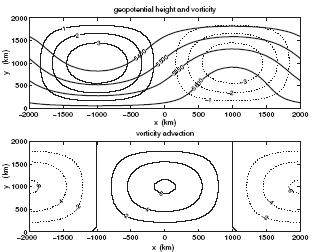
\includegraphics[!htp]{Fig_6_8Holt.jpg}
\caption{Uma típica figura}
\end{figure}


Donec arcu erat, eleifend in volutpat a, sodales ut leo. Nam vulputate ornare nisl, eget lobortis magna posuere a. Praesent sit amet est est, sit amet sollicitudin nibh. Nam sagittis nulla fermentum elit aliquet aliquet. Proin at sem vitae velit interdum viverra nec at diam. Aenean arcu dui, eleifend ut gravida ac, ornare placerat urna. Suspendisse aliquam condimentum metus nec faucibus. Lorem ipsum dolor sit amet, consectetur adipiscing elit. Aliquam non leo ipsum, sollicitudin consectetur mi. Duis erat eros, tempor in consequat in, scelerisque eget ante. Praesent placerat vulputate rhoncus. Ut et ante risus, et molestie felis.


\begin{figure}[!htp]
\centering
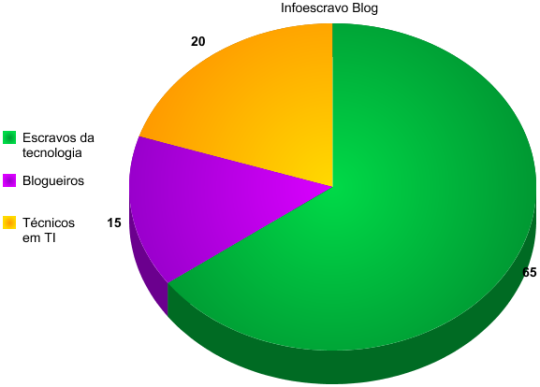
\includegraphics[scale = .5]{graficos-online-gratis.png}
\caption{Uma típica figura}
\end{figure}


Vivamus ultricies tincidunt lacus ut pharetra. Sed fringilla hendrerit tempus. Suspendisse potenti. Cras hendrerit tortor ac est condimentum pellentesque. Morbi pretium lectus nec sapien laoreet eu malesuada diam adipiscing. Aliquam nisl ipsum, fermentum ut aliquam nec, varius sit amet nisi. Pellentesque interdum cursus malesuada. Vestibulum ante ipsum primis in faucibus orci luctus et ultrices posuere cubilia Curae; Nullam malesuada bibendum tortor, ut bibendum lorem varius eu. In eros orci, volutpat ut facilisis sit amet, commodo quis nulla.


\begin{figure}[!htp]
\centering
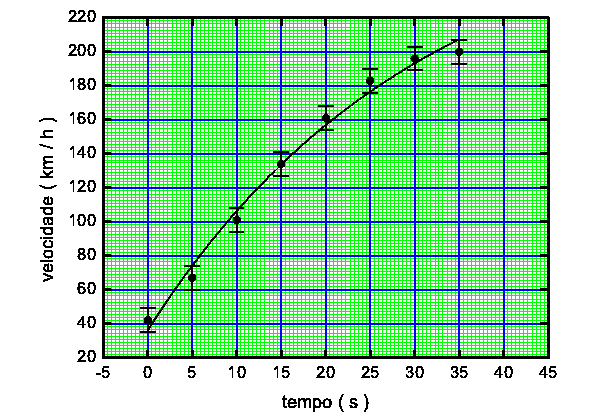
\includegraphics[scale = .5]{graf-fig1.png}
\caption{Uma típica figura}
\end{figure}



Sed lectus metus, mollis nec vulputate id, imperdiet eget urna. Nam ut dolor at metus venenatis suscipit et in ligula. In hac habitasse platea dictumst. Mauris scelerisque dolor sed nisl mattis accumsan. Aliquam vulputate placerat feugiat. Pellentesque faucibus neque mi. Etiam porttitor varius tempus. Mauris varius porttitor posuere. Pellentesque iaculis imperdiet lobortis. Sed vulputate purus nec felis rutrum molestie. 


\begin{figure}[!htp]
\centering
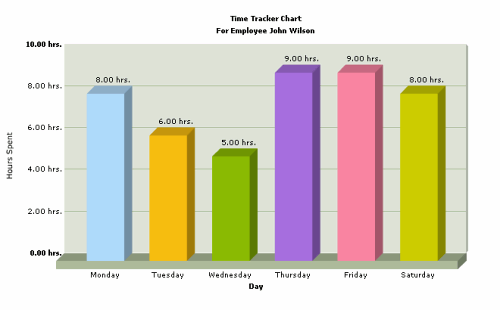
\includegraphics[!htp]{grafico}
\caption{Uma típica figura}
\end{figure}




%% T�tulo do Capitulo 4
\chapter{Título do Quarto Capítulo}
\label{cap:titulo do quarto capitulo}

Vivamus ultricies tincidunt lacus ut pharetra. Sed fringilla hendrerit tempus. Suspendisse potenti. Cras hendrerit tortor ac est condimentum pellentesque. Morbi pretium lectus nec sapien laoreet eu malesuada diam adipiscing. Aliquam nisl ipsum, fermentum ut aliquam nec, varius sit amet nisi. Pellentesque interdum cursus malesuada. Vestibulum ante ipsum primis in faucibus orci luctus et ultrices posuere cubilia Curae; Nullam malesuada bibendum tortor, ut bibendum lorem varius eu. In eros orci, volutpat ut facilisis sit amet, commodo quis nulla.

Sed lectus metus, mollis nec vulputate id, imperdiet eget urna. Nam ut dolor at metus venenatis suscipit et in ligula. In hac habitasse platea dictumst. Mauris scelerisque dolor sed nisl mattis accumsan. Aliquam vulputate placerat feugiat. Pellentesque faucibus neque mi. Etiam porttitor varius tempus. Mauris varius porttitor posuere. Pellentesque iaculis imperdiet lobortis. Sed vulputate purus nec felis rutrum molestie.


\section{Algoritmos}

\renewcommand{\baselinestretch}{0.5}  % distância entre linhas
\begin{codigo}[htb]
\fontsize{9pt}{9pt}\selectfont
      \begin{boxit}  % coloca o código dentro de um Box
      \vspace{2mm}
      \VerbatimInput[xleftmargin=8mm,numbers=left,obeytabs=true]{source/arquivo.cpp}
   \end{boxit}
   \caption{\it Código C++}
   \label{code:meu_codigo}
\end{codigo}


Nunc at fringilla dui. Pellentesque id tortor eu libero auctor rhoncus id vel velit. Duis auctor laoreet turpis, sed commodo tellus sollicitudin sit amet. Phasellus quis purus consectetur turpis hendrerit pretium eget in velit. Cras dignissim est vel mi malesuada a imperdiet velit condimentum. Vivamus ultrices diam non urna aliquet hendrerit. Sed lobortis, mauris quis egestas ullamcorper, nunc nulla auctor nulla, eu rutrum velit velit in nulla. Etiam lectus augue, pellentesque et porta at, pharetra id lectus. Duis eleifend eleifend mauris, nec mollis mauris vehicula nec. Nam sed ipsum ut massa lacinia vestibulum. Duis vitae sapien a lectus aliquam luctus eget sit amet nunc. Etiam a ipsum auctor tortor condimentum consectetur. Aliquam vestibulum libero sit amet nulla auctor aliquet. Sed laoreet imperdiet tellus non vulputate. Vivamus tristique ipsum vel metus venenatis in laoreet tortor hendrerit. Suspendisse potenti. Aenean tincidunt molestie libero sit amet porttitor. Class aptent taciti sociosqu ad litora torquent per conubia nostra, per inceptos himenaeos.


\renewcommand{\baselinestretch}{0.5}  % distância entre linhas
\begin{codigo}[htb]
\fontsize{9pt}{9pt}\selectfont
     \begin{boxit}  % coloca o código dentro de um Box
      \vspace{2mm}
      \VerbatimInput[xleftmargin=8mm,numbers=left,obeytabs=true]{calculadora.erl}
   \end{boxit}
   \caption{\it Código Erlang}
   \label{code:funcoes}
\end{codigo}


Cras nec quam mi, ut mattis ante. Lorem ipsum dolor sit amet, consectetur adipiscing elit. Sed fringilla auctor dictum. Nam hendrerit sapien sed massa consequat rutrum. Nullam congue, augue sed commodo malesuada, lectus nulla mollis magna, eget semper risus nisl eget elit. Duis vitae hendrerit massa. In a odio nunc, sit amet mollis dolor. In accumsan suscipit dui, a vestibulum diam condimentum ullamcorper. Etiam ut quam arcu, ac tristique ante. Vestibulum imperdiet elit non ante tristique accumsan. Donec vulputate fringilla tempor. Proin porttitor nisi nisi. Fusce vel ullamcorper orci. Lorem ipsum dolor sit amet, consectetur adipiscing elit. 

Vivamus ultricies tincidunt lacus ut pharetra. Sed fringilla hendrerit tempus. Suspendisse potenti. Cras hendrerit tortor ac est condimentum pellentesque. Morbi pretium lectus nec sapien laoreet eu malesuada diam adipiscing. Aliquam nisl ipsum, fermentum ut aliquam nec, varius sit amet nisi. Pellentesque interdum cursus malesuada. Vestibulum ante ipsum primis in faucibus orci luctus et ultrices posuere cubilia Curae; Nullam malesuada bibendum tortor, ut bibendum lorem varius eu. In eros orci, volutpat ut facilisis sit amet, commodo quis nulla.



% incluir referencias
\bibliography{tese}
\bibliographystyle{apa}


%\include{anexos}

\end{document}
